\documentclass{standalone}
\usepackage{tikz}
\usepackage{animate}
\usetikzlibrary{fit, positioning, arrows.meta, shapes.geometric, calc}

% 1. Create a savebox for the static background elements
\newsavebox{\staticbg}

\begin{document}

% 2. Draw the heavy static content exactly ONCE and save it to memory
\sbox{\staticbg}{%
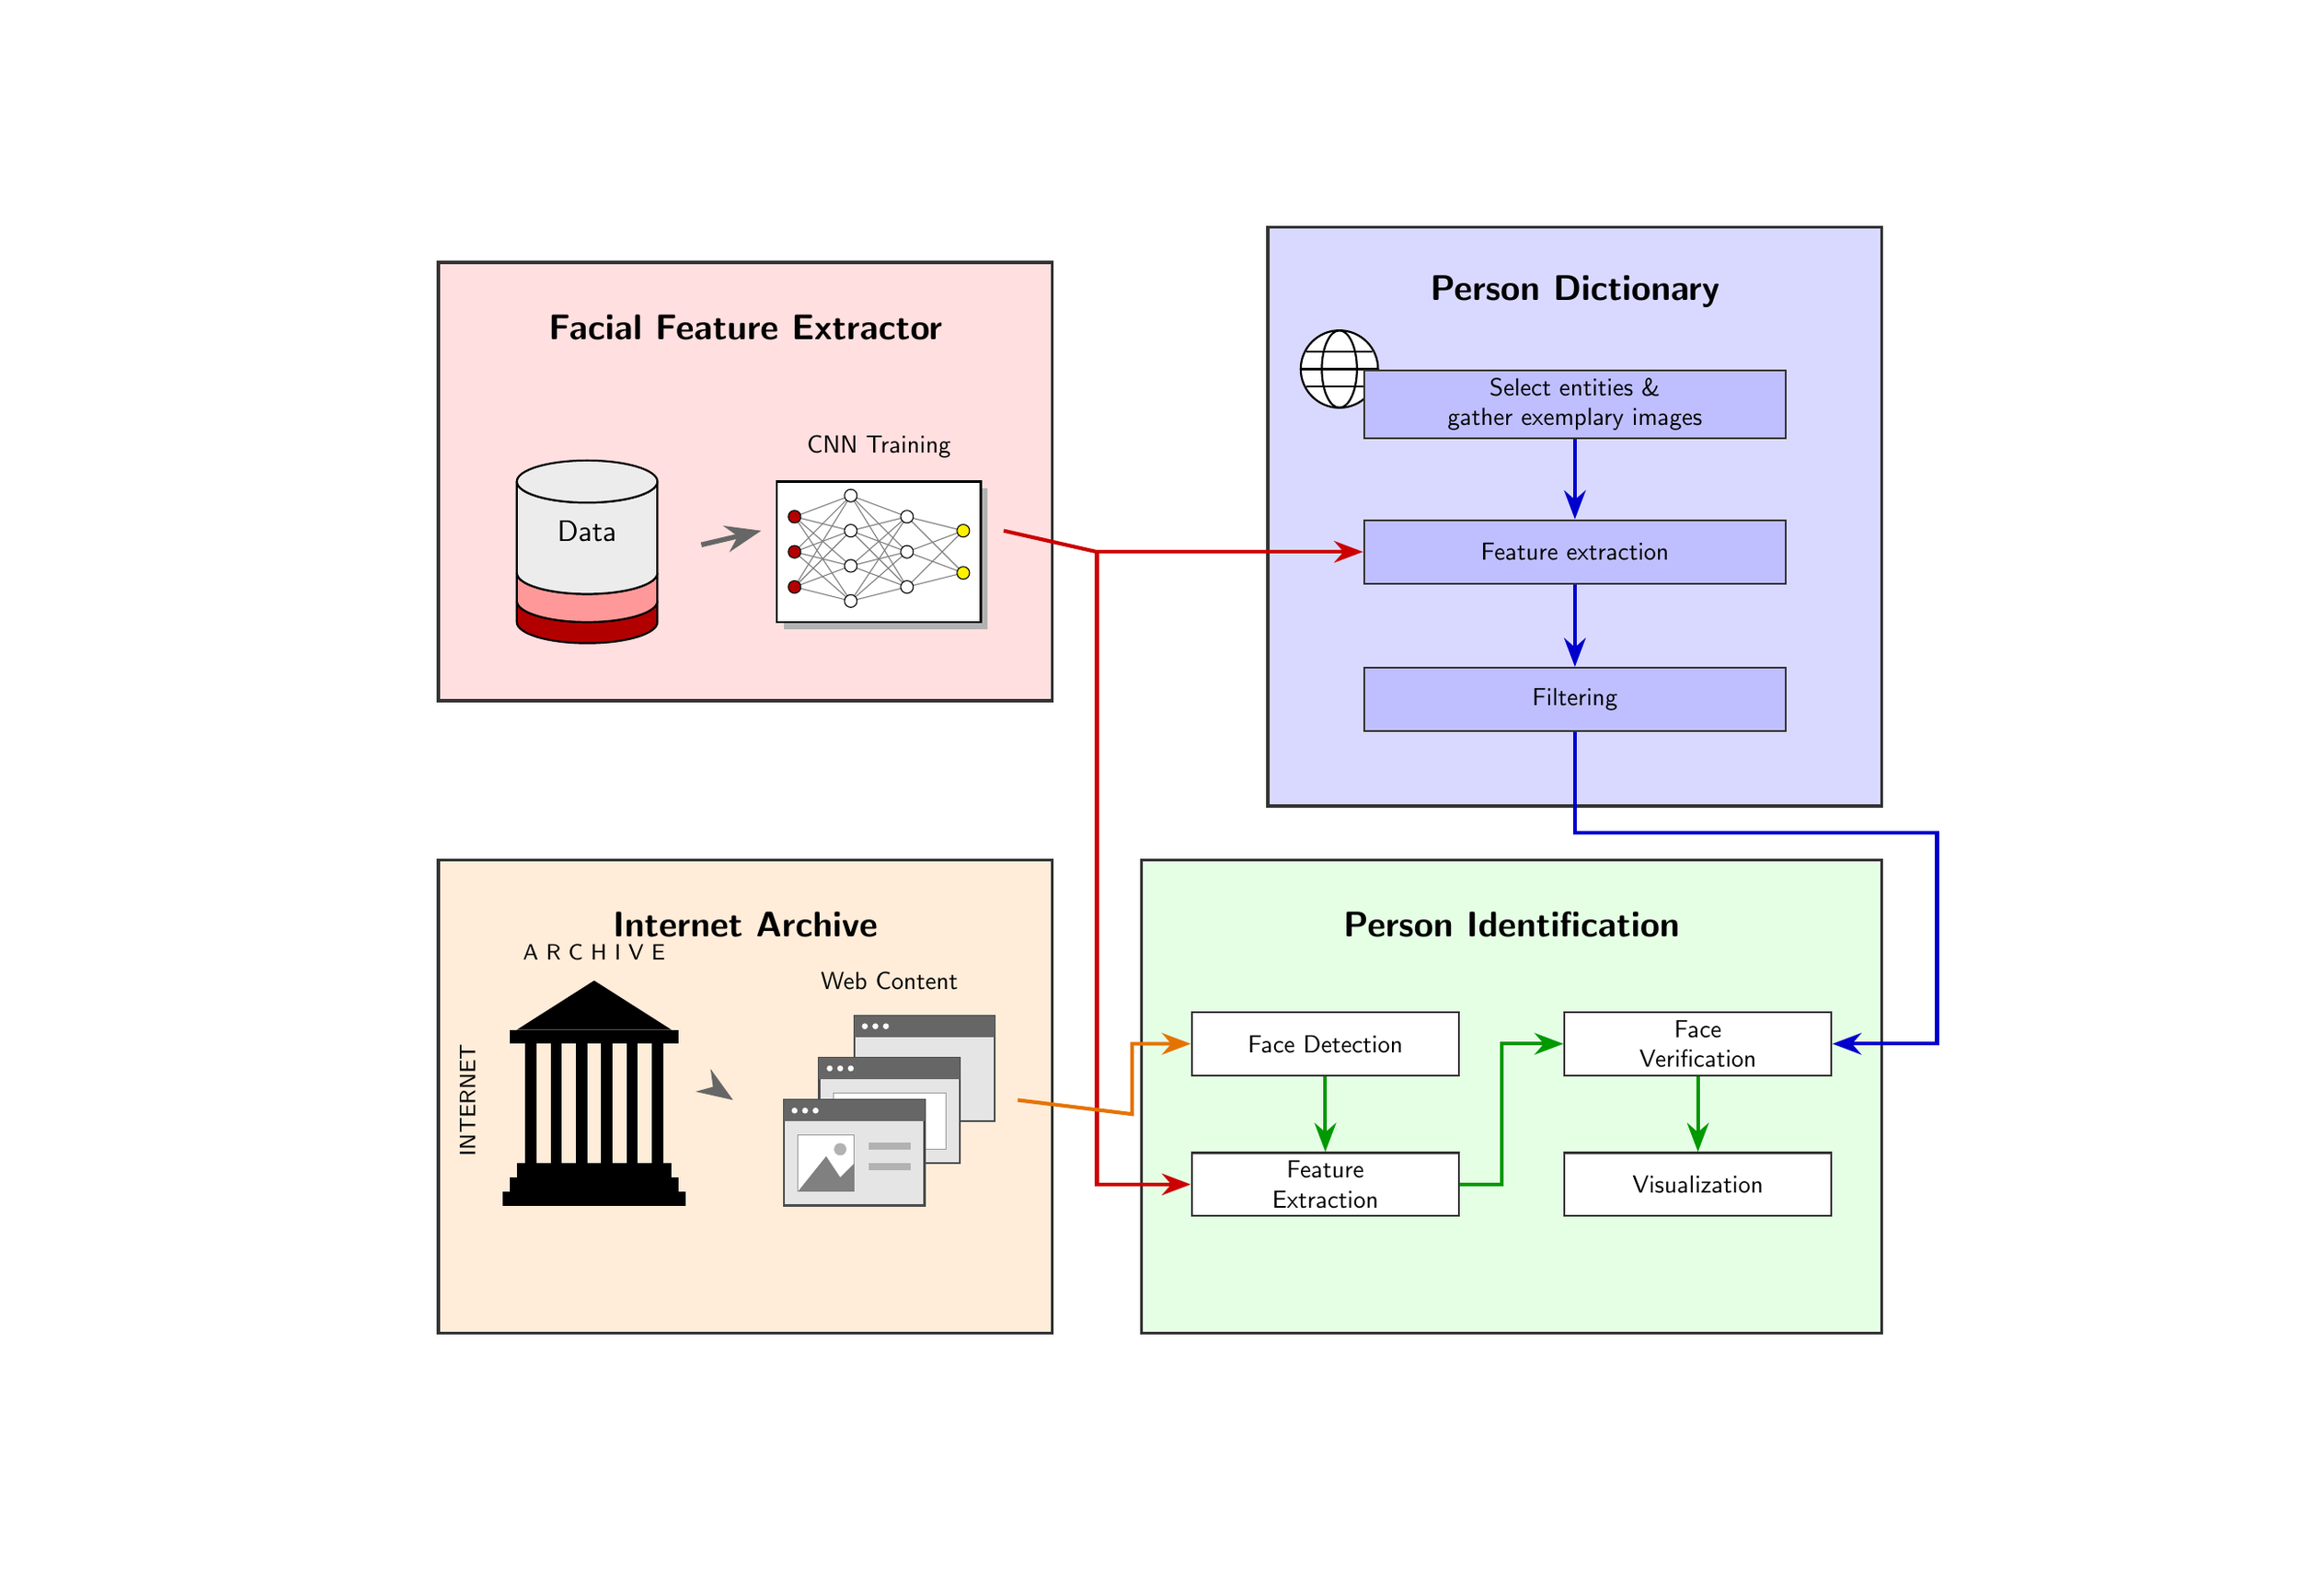
\begin{tikzpicture}[
    >=Stealth,
    % Parent Block Background Styles
    pink_bg/.style={fill=pink!50!white, draw=black!80, line width=1.2pt},
    blue_bg/.style={fill=blue!15!white, draw=black!80, line width=1.2pt},
    yellow_bg/.style={fill=orange!15!white, draw=black!80, line width=1.2pt},
    green_bg/.style={fill=green!10!white, draw=black!80, line width=1.2pt},
    % Inner Block Styles
    inner_box_blue/.style={fill=blue!25!white, draw=black!80, line width=0.8pt, minimum width=6cm, minimum height=0.9cm, align=center, font=\sffamily},
    inner_box_green/.style={fill=white, draw=black!80, line width=0.8pt, minimum width=3.8cm, minimum height=0.9cm, align=center, font=\sffamily},
    % Arrow Styles
    red_arrow/.style={draw=red!80!black, line width=1.5pt, -{Stealth[scale=1.2]}},
    blue_arrow/.style={draw=blue!80!black, line width=1.5pt, -{Stealth[scale=1.2]}},
    orange_arrow/.style={draw=orange!90!black, line width=1.5pt, -{Stealth[scale=1.2]}},
    green_arrow/.style={draw=green!60!black, line width=1.5pt, -{Stealth[scale=1.2]}},
    gray_arrow/.style={draw=black!60, line width=2pt, -{Stealth[scale=1.2]}}
]
    % Explicit Spacious Bounding Box
    \path [use as bounding box] (-6, -4) rectangle (26, 18);

    % =========================================================
    % BACKGROUND BOXES
    % =========================================================
    \coordinate (ff_tl) at (0, 14.5); \coordinate (ff_br) at (8.5, 8.5);
    \node[fit=(ff_tl) (ff_br), pink_bg] (ff_box) {};

    \coordinate (pd_tl) at (11.8, 15.0); \coordinate (pd_br) at (20.3, 7.0);
    \node[fit=(pd_tl) (pd_br), blue_bg] (pd_box) {};

    \coordinate (ia_tl) at (0, 6.0); \coordinate (ia_br) at (8.5, -0.5);
    \node[fit=(ia_tl) (ia_br), yellow_bg] (ia_box) {};

    \coordinate (pi_tl) at (10.0, 6.0); \coordinate (pi_br) at (20.3, -0.5);
    \node[fit=(pi_tl) (pi_br), green_bg] (pi_box) {};

    % =========================================================
    % BLOCK CONTENTS
    % =========================================================
    % --- A. Facial Feature Extractor ---
    \node[font=\Large\sffamily\bfseries] at (4.25, 13.7) {Facial Feature Extractor};

    \coordinate (data_tl) at (0.5, 12.0); \coordinate (data_br) at (3.5, 9.2);
    \draw[fill=red!70!black, thick] (1.0, 9.5) arc (180:360:1cm and 0.3cm) -- (3.0, 9.8) arc (360:180:1cm and 0.3cm) -- cycle;
    \draw[fill=pink!80!red, thick] (1.0, 9.8) arc (180:360:1cm and 0.3cm) -- (3.0, 10.2) arc (360:180:1cm and 0.3cm) -- cycle;
    \draw[fill=gray!15, thick] (1.0, 10.2) arc (180:360:1cm and 0.3cm) -- (3.0, 11.5) arc (360:180:1cm and 0.3cm) -- cycle;
    \draw[fill=gray!15, thick] (2.0, 11.5) ellipse (1cm and 0.3cm);
    \node[font=\large\sffamily] at (2.0, 10.8) {Data};
    \node[fit=(data_tl) (data_br)] (data_group) {};

    \coordinate (cnn_tl) at (4.6, 12.2); \coordinate (cnn_br) at (7.8, 9.4);
    \fill[black!30] (4.8, 9.4) rectangle (7.7, 11.4);
    \draw[fill=white, thick] (4.7, 9.5) rectangle (7.6, 11.5);
    \foreach \yA in {10.0, 10.5, 11.0} { \foreach \yB in {9.8, 10.3, 10.8, 11.3} { \draw[gray, thin] (4.95, \yA) -- (5.75, \yB); } }
    \foreach \yA in {9.8, 10.3, 10.8, 11.3} { \foreach \yB in {10.0, 10.5, 11.0} { \draw[gray, thin] (5.75, \yA) -- (6.55, \yB); } }
    \foreach \yA in {10.0, 10.5, 11.0} { \foreach \yB in {10.2, 10.8} { \draw[gray, thin] (6.55, \yA) -- (7.35, \yB); } }
    \foreach \y in {10.0, 10.5, 11.0} { \node[circle, draw=black, fill=red!70!black, inner sep=1.8pt] at (4.95, \y) {}; }
    \foreach \y in {9.8, 10.3, 10.8, 11.3} { \node[circle, draw=black, fill=white, inner sep=1.8pt] at (5.75, \y) {}; }
    \foreach \y in {10.0, 10.5, 11.0} { \node[circle, draw=black, fill=white, inner sep=1.8pt] at (6.55, \y) {}; }
    \foreach \y in {10.2, 10.8} { \node[circle, draw=black, fill=yellow, inner sep=1.8pt] at (7.35, \y) {}; }
    \node[font=\sffamily] at (6.15, 12.0) {CNN Training};
    \node[fit=(cnn_tl) (cnn_br)] (cnn_group) {};

    % --- B. Person Dictionary ---
    \node[font=\Large\sffamily\bfseries] at (16.05, 14.2) {Person Dictionary};

    \coordinate (globe_tl) at (12.0, 13.8); \coordinate (globe_br) at (13.4, 12.4);
    \draw[thick, fill=white] (12.7, 13.1) circle (0.55);
    \draw[thick] (12.7, 13.1) ellipse (0.25 and 0.55);
    \draw[thick] (12.15, 13.1) -- (13.25, 13.1);
    \draw[thick] (12.23, 13.35) -- (13.17, 13.35);
    \draw[thick] (12.23, 12.85) -- (13.17, 12.85);
    \node[fit=(globe_tl) (globe_br)] (globe_group) {};

    \node[inner_box_blue] (pd_b1) at (16.05, 12.6) {Select entities \& \\ gather exemplary images};
    \node[inner_box_blue] (pd_b2) at (16.05, 10.5) {Feature extraction};
    \node[inner_box_blue] (pd_b3) at (16.05, 8.4) {Filtering};

    \draw[blue_arrow] (pd_b1) -- (pd_b2); \draw[blue_arrow] (pd_b2) -- (pd_b3);

    % --- C. Internet Archive ---
    \node[font=\Large\sffamily\bfseries] at (4.25, 5.2) {Internet Archive};

    \coordinate (ia_logo_tl) at (0.0, 4.8); \coordinate (ia_logo_br) at (3.8, 0.8);
    \fill[black] (0.8, 1.2) rectangle (3.4, 1.4);
    \fill[black] (0.9, 1.4) rectangle (3.3, 1.6);
    \fill[black] (1.0, 1.6) rectangle (3.2, 1.8);
    \foreach \x in {1.20, 1.56, 1.92, 2.28, 2.64, 3.00} { \fill[black] (\x-0.08, 1.8) rectangle (\x+0.08, 3.5); }
    \fill[black] (0.9, 3.5) rectangle (3.3, 3.7);
    \fill[black] (1.0, 3.7) -- (3.2, 3.7) -- (2.1, 4.4) -- cycle;
    \node[rotate=90, font=\small\sffamily] at (0.3, 2.7) {INTERNET};
    \node[font=\small\sffamily] at (2.1, 4.8) {A R C H I V E};
    \node[fit=(ia_logo_tl) (ia_logo_br)] (ia_logo_group) {};

    \coordinate (web_tl) at (4.2, 4.6); \coordinate (web_br) at (8.0, 0.8);
    \fill[gray!20, draw=black!70, thick] (5.8, 2.4) rectangle (7.8, 3.9);
    \fill[black!60] (5.8, 3.6) rectangle (7.8, 3.9);
    \fill[white] (5.95, 3.75) circle (1.2pt); \fill[white] (6.1, 3.75) circle (1.2pt); \fill[white] (6.25, 3.75) circle (1.2pt);
    \fill[gray!20, draw=black!70, thick] (5.3, 1.8) rectangle (7.3, 3.3);
    \fill[black!60] (5.3, 3.0) rectangle (7.3, 3.3);
    \fill[white] (5.45, 3.15) circle (1.2pt); \fill[white] (5.6, 3.15) circle (1.2pt); \fill[white] (5.75, 3.15) circle (1.2pt);
    \fill[white, draw=black!40] (5.5, 2.0) rectangle (7.1, 2.8);
    \fill[gray!20, draw=black!70, thick] (4.8, 1.2) rectangle (6.8, 2.7);
    \fill[black!60] (4.8, 2.4) rectangle (6.8, 2.7);
    \fill[white] (4.95, 2.55) circle (1.2pt); \fill[white] (5.1, 2.55) circle (1.2pt); \fill[white] (5.25, 2.55) circle (1.2pt);
    \fill[white, draw=black!40] (5.0, 1.4) rectangle (5.8, 2.2);
    \fill[black!30] (5.6, 2.0) circle (2.5pt); 
    \fill[black!50] (5.0, 1.4) -- (5.4, 1.9) -- (5.6, 1.6) -- (5.8, 1.8) -- (5.8, 1.4) -- cycle; 
    \fill[black!30] (6.0, 2.0) rectangle (6.6, 2.1);
    \fill[black!30] (6.0, 1.7) rectangle (6.6, 1.8);
    \node[font=\sffamily] at (6.3, 4.4) {Web Content};
    \node[fit=(web_tl) (web_br)] (web_group) {};

    % --- D. Person Identification ---
    \node[font=\Large\sffamily\bfseries] at (15.15, 5.2) {Person Identification};

    \node[inner_box_green] (pi_b1) at (12.5, 3.5) {Face Detection};
    \node[inner_box_green] (pi_b2) at (12.5, 1.5) {Feature\\Extraction};
    \node[inner_box_green] (pi_b3) at (17.8, 3.5) {Face\\Verification};
    \node[inner_box_green] (pi_b4) at (17.8, 1.5) {Visualization};

    \draw[green_arrow] (pi_b1) -- (pi_b2);
    \draw[green_arrow] (pi_b2.east) -- ++(0.6,0) |- (pi_b3.west);
    \draw[green_arrow] (pi_b3) -- (pi_b4);

    % =========================================================
    % GLOBAL ROUTING ARROWS
    % =========================================================
    \draw[gray_arrow] (data_group.east) -- (cnn_group.west);
    \draw[gray_arrow] (ia_logo_group.east) -- (web_group.west);

    \coordinate (red_split) at (9.25, 10.5);
    \draw[red_arrow, -] (cnn_group.east) -- (red_split);
    \draw[red_arrow] (red_split) |- (pd_b2.west);
    \draw[red_arrow] (red_split) |- (pi_b2.west);

    \draw[orange_arrow] (web_group.east) -- (9.75, 2.5) |- (pi_b1.west);
    \draw[blue_arrow] (pd_b3.south) -- (16.05, 6.5) -- (21.2, 6.5) |- (pi_b3.east);
\end{tikzpicture}%
} % End of savebox


% 3. Animate over the static background
\begin{animateinline}[controls, loop]{3}
\multiframe{61}{iFrame=0+1}{%
\begin{tikzpicture}
    % Ensure exactly the same bounding box as the parent savebox
    \path [use as bounding box] (-6, -4) rectangle (26, 18);
    
    % Stamp the fully rendered background into the frame
    \node[anchor=south west, inner sep=0pt, outer sep=0pt] at (-6, -4) {\usebox{\staticbg}};

    % =========================================================
    % Reconstruct dummy node boxes purely for geometry routing
    % (These invisible nodes provide the hooks for the fit box)
    % =========================================================
    \coordinate (ff_tl) at (0, 14.5); \coordinate (ff_br) at (8.5, 8.5);
    \node[fit=(ff_tl) (ff_br), inner sep=0pt] (ff_box) {};

    \coordinate (data_tl) at (0.5, 12.0); \coordinate (data_br) at (3.5, 9.2);
    \node[fit=(data_tl) (data_br), inner sep=0pt] (data_group) {};

    \coordinate (cnn_tl) at (4.6, 12.2); \coordinate (cnn_br) at (7.8, 9.4);
    \node[fit=(cnn_tl) (cnn_br), inner sep=0pt] (cnn_group) {};

    \coordinate (pd_tl) at (11.8, 15.0); \coordinate (pd_br) at (20.3, 7.0);
    \node[fit=(pd_tl) (pd_br), inner sep=0pt] (pd_box) {};

    \coordinate (globe_tl) at (12.0, 13.8); \coordinate (globe_br) at (13.4, 12.4);
    \node[fit=(globe_tl) (globe_br), inner sep=0pt] (globe_group) {};

    \node[minimum width=6cm, minimum height=0.9cm] (pd_b1) at (16.05, 12.6) {};
    \node[minimum width=6cm, minimum height=0.9cm] (pd_b2) at (16.05, 10.5) {};
    \node[minimum width=6cm, minimum height=0.9cm] (pd_b3) at (16.05, 8.4) {};

    \coordinate (ia_tl) at (0, 6.0); \coordinate (ia_br) at (8.5, -0.5);
    \node[fit=(ia_tl) (ia_br), inner sep=0pt] (ia_box) {};

    \coordinate (ia_logo_tl) at (0.0, 4.8); \coordinate (ia_logo_br) at (3.8, 0.8);
    \node[fit=(ia_logo_tl) (ia_logo_br), inner sep=0pt] (ia_logo_group) {};

    \coordinate (web_tl) at (4.2, 4.6); \coordinate (web_br) at (8.0, 0.8);
    \node[fit=(web_tl) (web_br), inner sep=0pt] (web_group) {};

    \coordinate (pi_tl) at (10.0, 6.0); \coordinate (pi_br) at (20.3, -0.5);
    \node[fit=(pi_tl) (pi_br), inner sep=0pt] (pi_box) {};

    \node[minimum width=3.8cm, minimum height=0.9cm] (pi_b1) at (12.5, 3.5) {};
    \node[minimum width=3.8cm, minimum height=0.9cm] (pi_b2) at (12.5, 1.5) {};
    \node[minimum width=3.8cm, minimum height=0.9cm] (pi_b3) at (17.8, 3.5) {};
    \node[minimum width=3.8cm, minimum height=0.9cm] (pi_b4) at (17.8, 1.5) {};

    % Extract Keyframes from original nodes
    \path (ff_box.north west) coordinate (kf0_tl) (ff_box.south east) coordinate (kf0_br);
    \path (data_group.north west) coordinate (kf1_tl) (data_group.south east) coordinate (kf1_br);
    \path (cnn_group.north west) coordinate (kf2_tl) (cnn_group.south east) coordinate (kf2_br);
    \path (pd_box.north west) coordinate (kf3_tl) (pd_box.south east) coordinate (kf3_br);
    \path (globe_group.north west) coordinate (kf4_tl) (globe_group.south east) coordinate (kf4_br);
    \path (pd_b1.north west) coordinate (kf5_tl) (pd_b1.south east) coordinate (kf5_br);
    \path (pd_b2.north west) coordinate (kf6_tl) (pd_b2.south east) coordinate (kf6_br);
    \path (pd_b3.north west) coordinate (kf7_tl) (pd_b3.south east) coordinate (kf7_br);
    \path (ia_box.north west) coordinate (kf8_tl) (ia_box.south east) coordinate (kf8_br);
    \path (ia_logo_group.north west) coordinate (kf9_tl) (ia_logo_group.south east) coordinate (kf9_br);
    \path (web_group.north west) coordinate (kf10_tl) (web_group.south east) coordinate (kf10_br);
    \path (pi_box.north west) coordinate (kf11_tl) (pi_box.south east) coordinate (kf11_br);
    \path (pi_b1.north west) coordinate (kf12_tl) (pi_b1.south east) coordinate (kf12_br);
    \path (pi_b2.north west) coordinate (kf13_tl) (pi_b2.south east) coordinate (kf13_br);
    \path (pi_b3.north west) coordinate (kf14_tl) (pi_b3.south east) coordinate (kf14_br); 
    \path (pi_b4.north west) coordinate (kf15_tl) (pi_b4.south east) coordinate (kf15_br);

    % Determine transition parameters
    \pgfmathsetmacro{\framesPerTrans}{4}
    \pgfmathtruncatemacro{\currentTrans}{min(15, \iFrame / \framesPerTrans)} 
    \pgfmathsetmacro{\localProg}{mod(\iFrame, \framesPerTrans) / \framesPerTrans}

    % Interpolate between keyframes
    \ifcase\currentTrans
        \coordinate (curr_tl) at ($(kf0_tl)!\localProg!(kf1_tl)$);
        \coordinate (curr_br) at ($(kf0_br)!\localProg!(kf1_br)$);
    \or
        \coordinate (curr_tl) at ($(kf1_tl)!\localProg!(kf2_tl)$);
        \coordinate (curr_br) at ($(kf1_br)!\localProg!(kf2_br)$);
    \or
        \coordinate (curr_tl) at ($(kf2_tl)!\localProg!(kf3_tl)$);
        \coordinate (curr_br) at ($(kf2_br)!\localProg!(kf3_br)$);
    \or
        \coordinate (curr_tl) at ($(kf3_tl)!\localProg!(kf4_tl)$);
        \coordinate (curr_br) at ($(kf3_br)!\localProg!(kf4_br)$);
    \or
        \coordinate (curr_tl) at ($(kf4_tl)!\localProg!(kf5_tl)$);
        \coordinate (curr_br) at ($(kf4_br)!\localProg!(kf5_br)$);
    \or
        \coordinate (curr_tl) at ($(kf5_tl)!\localProg!(kf6_tl)$);
        \coordinate (curr_br) at ($(kf5_br)!\localProg!(kf6_br)$);
    \or
        \coordinate (curr_tl) at ($(kf6_tl)!\localProg!(kf7_tl)$);
        \coordinate (curr_br) at ($(kf6_br)!\localProg!(kf7_br)$);
    \or
        \coordinate (curr_tl) at ($(kf7_tl)!\localProg!(kf8_tl)$);
        \coordinate (curr_br) at ($(kf7_br)!\localProg!(kf8_br)$);
    \or
        \coordinate (curr_tl) at ($(kf8_tl)!\localProg!(kf9_tl)$);
        \coordinate (curr_br) at ($(kf8_br)!\localProg!(kf9_br)$);
    \or
        \coordinate (curr_tl) at ($(kf9_tl)!\localProg!(kf10_tl)$);
        \coordinate (curr_br) at ($(kf9_br)!\localProg!(kf10_br)$);
    \or
        \coordinate (curr_tl) at ($(kf10_tl)!\localProg!(kf11_tl)$);
        \coordinate (curr_br) at ($(kf10_br)!\localProg!(kf11_br)$);
    \or
        \coordinate (curr_tl) at ($(kf11_tl)!\localProg!(kf12_tl)$);
        \coordinate (curr_br) at ($(kf11_br)!\localProg!(kf12_br)$);
    \or
        \coordinate (curr_tl) at ($(kf12_tl)!\localProg!(kf13_tl)$);
        \coordinate (curr_br) at ($(kf12_br)!\localProg!(kf13_br)$);
    \or
        \coordinate (curr_tl) at ($(kf13_tl)!\localProg!(kf14_tl)$);
        \coordinate (curr_br) at ($(kf13_br)!\localProg!(kf14_br)$);
    \or
        \coordinate (curr_tl) at ($(kf14_tl)!\localProg!(kf15_tl)$);
        \coordinate (curr_br) at ($(kf14_br)!\localProg!(kf15_br)$);
    \else
        \coordinate (curr_tl) at (kf15_tl);
        \coordinate (curr_br) at (kf15_br);
    \fi

    % SOLID RED BOUNDING BOX
    \node[draw=red, line width=3pt, inner sep=5pt, rounded corners=2pt, fit=(curr_tl) (curr_br)] {};

\end{tikzpicture}%
}
\end{animateinline}
\end{document}